\appendix
\chapter{Appendix}

\section{Program Implementation}
The implementation was done using MATLAB 2012b. In order to run the program implementation the image processing toolbox needs to be installed. The source code for the COSFIRE filter, around which this approach was developed, was provided \footnotemark by Dr. George Azzopardi. It is included in the CD along with the other scripts. \\

\footnotetext[1]{Taken From \url{http://matlabserver.cs.rug.nl/cosfireweb/web/index.html}}

The following subsections include a detailed description of each developed script along with it's code.

\label{sec:built}
\subsection{ExperimentParameters.m}
\subsubsection{Description}
The "ExperimentParameters.m" script contains a list of variables which control the experiment's execution. The following is a description of each of these variables.

\begin{enumerate}
\item {\bf LoadConfigurationFromFile}
    \begin{itemize}
        \item Boolean switch which determines whether to load the configuration file from disk or not
    \end{itemize}
\item {\bf loadTrainingFromFile}
    \begin{itemize}
        \item Boolean switch which determines whether to load the training file from disk or not
    \end{itemize}
\item {\bf NFiltersPerProtoType}
    \begin{itemize}
        \item Determines the number of COSFIRE filters to configure for each model symbol.
    \end{itemize}
\item {\bf minNumberOfTuplesPerFilter}
    \begin{itemize}
        \item Determines the minimum number of tuples that must be achieved for each configured COSFIRE filters.
    \end{itemize}
\item {\bf minNumberOfDistinctOrientationsPerFilter}
    \begin{itemize}
        \item Determines the minimum number of unique orientations detected for each configured COSFIRE filters.
    \end{itemize}
\item {\bf OS}
    \begin{itemize}
        \item Determines which OS is being used, so as to switch between different path strings.
    \end{itemize}
\item {\bf ModelsFolder}
    \begin{itemize}
        \item Specifies the name of the folder in which the model symbols are found
    \end{itemize}
\item {\bf ModelsExtension}
    \begin{itemize}
        \item Specifies the model symbols' file extension
    \end{itemize}
\item {\bf TestingFolder}
    \begin{itemize}
        \item Specifies the name of the folder in which the testing symbols are found
    \end{itemize}
\item {\bf TestingExtension}
    \begin{itemize}
        \item Specifies the testing symbols' file extension
    \end{itemize}
\item {\bf WIN/OSX.COSFIREFolder}
    \begin{itemize}
        \item Specifies the folder in which the COSFIRE filter code resides
    \end{itemize}
\item {\bf WIN/OSX.GaborFolder}  
    \begin{itemize}
        \item Specifies the folder in which the Gabor filter code resides
    \end{itemize}   
\item {\bf WIN/OSX.DataSetsPath}
    \begin{itemize}
        \item Specifies the path in which the data sets are found.
    \end{itemize}
\item {\bf WIN/OSX.ModelsDirectory}
    \begin{itemize}
        \item Specifies the path in which the model symbols are found
    \end{itemize}
\item {\bf WIN/OSX.TestingDirectory}
    \begin{itemize}
        \item Specifies the path in which the test symbols are found
    \end{itemize}
\end{enumerate}
\subsubsection{Code}
The code for this script is found on the next page.
\vspace{120.55mm}



\subsection{Utilities.m}
\subsubsection{Description}
The "Utilities.m" script contains a list of functions which are used through out the remaining scripts of the experiment. The following is a list of all the available functions alongside a description of what they do:

\begin{enumerate}
    \item {\bf SaveOperators()}
    \begin{itemize}
        \item Saves a visualisation of the configured operator to file
    \end{itemize}
    \item {\bf saveFalsePositive()}
    \begin{itemize}
        \item Saves a visualisation of the failed recognitions to file
    \end{itemize}
    \item {\bf printRhoList()}
    \begin{itemize}
        \item Saves a visualisation of the selected rho list on the model image
    \end{itemize}
    \item {\bf rhoAnalyser()}
    \begin{itemize}
        \item Analyses the selected rho list against all the models to check whether all models can be properly configured
    \end{itemize}
    \item {\bf SetupFolderEnviroment()}
    \begin{itemize}
        \item Sets up directories in which to save files etc.
    \end{itemize}
    \item {\bf createResultFolder()}
    \begin{itemize}
        \item Creates a result folder in which to dump the results file
    \end{itemize}
    \item {\bf createIntermediateFolder()}
    \begin{itemize}
        \item Creates an intermediate folder in which checkpoints are saved to disk.
    \end{itemize}
    \item {\bf ReadXMLV1()}
    \begin{itemize}
        \item Reads the XML file for the first category of datasets in order to determine if the recognition was a successful one or not.
    \end{itemize}
    \item {\bf ReadXMLV2()}
    \begin{itemize}
        \item Reads the XML file for the second and third category of datasets in order to determine if the recognition was a successful one or not.
    \end{itemize}
    \item {\bf writeTrainingData()}
    \begin{itemize}
        \item Write the training data(feature vectors) to an excel file
    \end{itemize}
    \item {\bf visualizeTrainingData()}
    \begin{itemize}
        \item Saves a visualisation of all the feature vectors togather
    \end{itemize}
    \item {\bf appendElapsedTimeToFile()}
    \begin{itemize}
        \item Adds the elapsed time to the final result
    \end{itemize}
    \item {\bf appendTPFP()}
    \begin{itemize}
        \item Saves to file the true positives or false positives
    \end{itemize}
    \item {\bf appendResultToFile()}
    \begin{itemize}
        \item Saves to file the final result for the experiment
    \end{itemize}
    \item {\bf getCOSFIREFolder()}
    \begin{itemize}
        \item Gets the folder in which the COSFIRE filter code resides
    \end{itemize}
    \item {\bf getGaborFolder()}
    \begin{itemize}
        \item Gets the folder in which the Gabor filter code resides
    \end{itemize}
    \item {\bf getModelsDirectory()}
    \begin{itemize}
        \item Gets the directory in which the models reside
    \end{itemize}
    \item {\bf getTestingDirectory()}
    \begin{itemize}
        \item Gets the directory in which the testing images reside
    \end{itemize}
    \item {\bf Signal()}
    \begin{itemize}
        \item Gives a signal when the experiment is done.
    \end{itemize}    
\end{enumerate}
\subsubsection{Code}
The code for this script is found on the next page.
\vspace{133.3mm}



\subsection{ConfigureOperators.m}
\subsubsection{Description}
The "ConfigureOperators.m" script contains the logic by which for every model symbol in a dataset a number of COSFIRE filters are applied. This outputs a collection of COSFIRE operators which are then passed to the "TrainOperators.m" script.
\subsubsection{Code}
The code for this script is found on the next page.
\vspace{133.3mm}

\subsection{TrainOperators.m}
\subsubsection{Description}
The "TrainOperators.m" script contains the logic by which for every model symbol in a dataset, every COSFIRE operator yielded from the "ConfigureOperators.m" script, is re-applied. This outputs a collection of feature vectors describing each model, which are then passed to the "TestOperators.m" script.
\subsubsection{Code}
The code for this script is found on the next page.
\vspace{133.3mm}

\subsection{TestOperators.m}
\subsubsection{Description}
The "TestOperators.m" script contains the logic by which every test image in the dataset has a number of COSFIRE filters applied to it from which a feature vector is yielded. This feature vector is the cross referenced against the collection of feature vectors yielded from the "TrainOperators.m" script. For every test image, its corresponding XML file is read to determine whether it is a true positive or a false positive.

\subsubsection{Code}
The code for this script is found on the next page.
\vspace{133.3mm}


\subsection{Experiment.m}
\subsubsection{Description}
The "Experiment.m" script contains the logic by which the whole experiment is run. It calls the other scripts in order to successfully execute an experiment.

\subsubsection{Code}
The code for this script is found on the next page.
\vspace{133.3mm}

\section{CD Contents}
\label{sec:CD}
Further to this report, a CD was created containing other information that could not be included in this report. The following are the contents of the CD.

\subsection{Dissertation document}
The following two document formats of the dissertation are available on the CD

    \begin{enumerate}
        \item /Report/LukeAgius-080358084-Dissertation.pdf
    \end{enumerate}

\subsection{Video}
In the case of MATLAB IDE not being available for the reviewer of this project, a video has been added which shows the setup and execution of an experiment which is found in:
            \begin{itemize}
                  \item /Video/SampleRun.mov
            \end{itemize}

This sample experiment run shows the successful classification of 50 test images for the most simple dataset.

\subsection{Implementation}
A full implementation has been included in the CD which consists of:

    \begin{enumerate}
        \item COSFIRE Filter code
            \begin{itemize}
              \item Implementation/COSFIREFilter/\ldots
            \end{itemize}
        \item Matlab Scripts
            \begin{itemize}
                  \item Implementation/Scripts/ExperimentParameters.m
                  \item Implementation/Scripts/Utilities.m
                  \item Implementation/Scripts/ConfigureOperators.m
                  \item Implementation/Scripts/TrainOperators.m
                  \item Implementation/Scripts/TestOperators.m
                  \item Implementation/Scripts/Experiment.m
            \end{itemize}
    \end{enumerate}

\subsection{Datasets}
The datasets used for this dissertation have been included in the CD as well. The following tables, A.1 and A.2, list all the included datasets.

\begin{table}[H]
\centering
\caption[List of all datasets available in the CD]{Available datasets in the CD}
\begin{tabular}{ccccccccccccccc}
  \hline
      Category no. & & Dataset name & & & Path \\
  \hline
  
      1 & & Sketches25f-Level1 & & & /Datasets/Category1/Sketches25f-Level1/  \\
      1 & & Sketches25f-Level2 & & & /Datasets/Category1/Sketches25f-Level2/  \\
      1 & & Sketches25f-Level3 & & & /Datasets/Category1/Sketches25f-Level3/  \\
      1 & & Sketches25-Level1  & & & /Datasets/Category1/Sketches25-Level1/  \\
      1 & & Sketches25-Level2  & & & /Datasets/Category1/Sketches25-Level2/  \\
      1 & & Sketches25-Level3  & & & /Datasets/Category1/Sketches25-Level3/  \\
      1 & & Sketches50f-Level1 & & & /Datasets/Category1/Sketches50f-Level1/ \\
      1 & & Sketches50f-Level2 & & & /Datasets/Category1/Sketches50f-Level2/  \\
      1 & & Sketches50f-Level3 & & & /Datasets/Category1/Sketches50f-Level3/  \\
      1 & & Sketches50-Level1  & & & /Datasets/Category1/Sketches50-Level1/  \\
      1 & & Sketches50-Level2  & & & /Datasets/Category1/Sketches50-Level2/  \\
      1 & & Sketches50-Level3  & & & /Datasets/Category1/Sketches50-Level3/  \\      
      1 & & Sketches100f-Level1 & & & /Datasets/Category1/Sketches100f-Level1/  \\
      1 & & Sketches100f-Level2 & & & /Datasets/Category1/Sketches100f-Level2/  \\
      1 & & Sketches100f-Level3 & & & /Datasets/Category1/Sketches100f-Level3/  \\
      1 & & Sketches100-Level1 & & & /Datasets/Category1/Sketches100-Level1/  \\
      1 & & Sketches100-Level2 & & & /Datasets/Category1/Sketches100-Level2/  \\
      1 & & Sketches100-Level3 & & & /Datasets/Category1/Sketches100-Level3/  \\      
      1 & & Sketches150f-Level1 & & & /Datasets/Category1/Sketches150f-Level1/   \\
  \hline
\end{tabular}
\end{table}
\vspace{49.3mm}



\begin{table}[H]
\centering
\caption[List of all datasets available in the CD]{Available datasets in the CD}
\begin{tabular}{ccccccccccccccc}
  \hline
      Category & & Name & & & Path \\
  \hline
      1 & & Sketches150f-Level2 & & & /Datasets/Category1/Sketches150f-Level2/ \\
      1 & & Sketches150f-Level3 & & & /Datasets/Category1/Sketches150f-Level3/  \\
      1 & & Sketches150-Level1 & & & /Datasets/Category1/Sketches150-Level1/  \\
      1 & & Sketches150-Level2 & & & /Datasets/Category1/Sketches150-Level2/  \\
      1 & & Sketches150-Level3 & & & /Datasets/Category1/Sketches150-Level3/  \\
      2 & & Rotation & & & /Datasets/Category2/Rotation/  \\
      2 & & Scaling & & & /Datasets/Category2/Scaling/  \\
      2 & & RotationScaling & & & /Datasets/Category2/RotatingScaling/  \\
      3 & & Noise A & & & /Datasets/Category3/NoiseA/  \\
      3 & & Noise B & & & /Datasets/Category3/NoiseB/  \\
      3 & & Noise E & & & /Datasets/Category3/NoiseE/  \\
      4 & & setA & & & /Datasets/Category4/SetA/  \\
      4 & & setB & & & /Datasets/Category4/SetB/  \\
      4 & & setC & & & /Datasets/Category4/SetC/  \\
  \hline
\end{tabular}
\end{table}
\vspace{65.3mm}


\section{How to run an experiment}
\label{sec:howto}
Before running an experiment, the necessary scripts and files must be copied to disk in a dedicated directory. The following walkthrough is an example of how to setup an experiment for a windows environment.

\subsection{File And Directory Setup}

First, create a new directory called "Experiment" anywhere you like. In this folder copy the, "Datasets" and "Implementation" folders from the CD contents. The datasets folder holds the images that the experiment will go through while the implementation folder contains the experiment's scripts. The directory structure should look as follows:

\begin{itemize}
    \item C:\textbackslash Experiment\textbackslash
    \item C:\textbackslash Experiment\textbackslash Datasets\textbackslash
    \item C:\textbackslash Experiment\textbackslash Implementation\textbackslash
\end{itemize}

Once that the directories has been set up and the correct files have been copied to those directories open MATLAB. Once MATLAB has been opened, input the path "C:\textbackslash Experiment\textbackslash Implementation\textbackslash" in the Address field as shown in the following figure, Fig. \ref{fig:address}:

\begin{figure*}[h]
        \centering
        \fbox{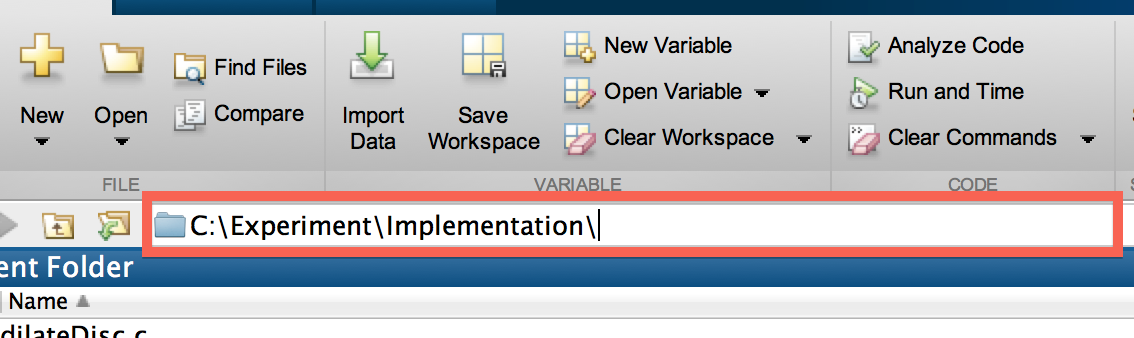
\includegraphics[width=0.8\textwidth]{figures/Howto/fieldAddress.png}}
        \caption[Inserting correct path in MATLAB address field]{}
        \label{fig:address}
\end{figure*}

Once that the correct path has been inputted in MATLAB's address field, the following files should be displayed in MATLAB's current folder section , Fig. \ref{fig:currentfolder}.

\begin{figure*}[h]
        \centering
        \fbox{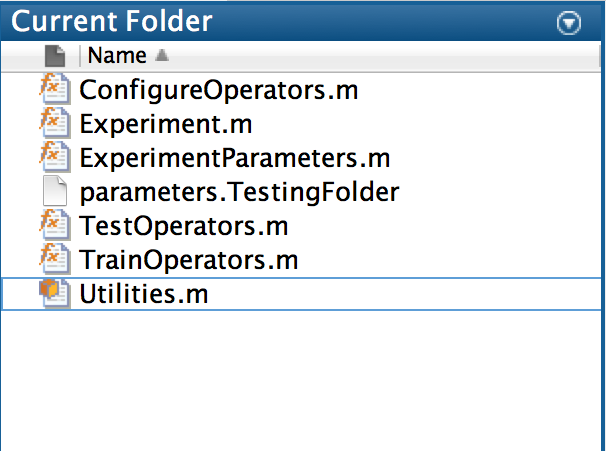
\includegraphics[width=0.5\textwidth]{figures/Howto/currentFolder.png}}
        \caption[Current Folder after inserting the correct path in MATLAB address field]{}
        \label{fig:currentfolder}
\end{figure*}

Upon, having the correct "Current Folder" setup in MATLAB, continue by double clicking the script with the name "ExperimentParameters.m". This will open the parameters script for the experiment. In the next subsection we explain how to set up the parameters for an experiment.

\subsection{Parameter Setup}
Prior to the execution of an experiment, the parameters in the ExperimentParameters.m script must be setup properly. The first parameters that need to be set are the check point parameters. These parameters will determine whether the configuration or the training file should be loaded from disk or generated. The following is an example:\\

\begin{lstlisting}
params.loadConfigurationFromFile  = 1; 
params.loadTrainingFromFile       = 1;
\end{lstlisting}

The next parameters that should be set up are the NFiltersPerProtoType, minNumberOfTuplesPerFilter, and minNumberOfDistinctOrientationsPerFilter parameters. The following example we are instructing the code to create three filters for each symbol from which five tuples and two distinct orientations must be created at minimum.\\

\begin{lstlisting}
params.NFiltersPerProtoType                       = 3;
params.minNumberOfTuplesPerFilter                 = 5;
params.minNumberOfDistinctOrientationsPerFilter   = 2;
\end{lstlisting}

Next, the type of OS needs to be specified. The permitted values for this parameter are "OSX" or "WIN". Each value correspond to either an Apple OSX or a Microsoft Windows environment. Afterwards we need to specify the directory path for the COSFIRE filter folder and that of the Gabor filters as well. Along with these paths, we need to also specify where the datasets are currently situated.\\

\begin{lstlisting}
params.OS                        = 'WIN';
params.WIN.COSFIREFolder         = 'C:\COSFIREFilter\COSFIRE\';
params.WIN.GaborFolder           = 'C:\COSFIREFilter\Gabor\'; 
params.WIN.DataSetsPath          = 'C:\Datasets\Category 1\';
\end{lstlisting}

Finally, the name of the folders in which the model and test symbols reside needs to be specified. Along with this the extension file for each set of symbols needs to be specified as well. In the following example, we are specifying that the models folder is called 'models' which contains files of the type '.tif' and that the testing images folder is called 'NoiseB' which contains files of the type '.tiff' \\

\begin{lstlisting}
params.ModelsFolder                 = 'models';
params.ModelsExtension              = '.tif';
params.TestingFolder                = 'NoiseB';
params.TestingExtension             = '.tiff';
\end{lstlisting}

Note, that these names must correspond to the same folder names in the the dataset that is to be executed.

\subsection{Execution}
Once that the environment parameters are set up correctly, the following command needs to be entered in the MATLAB command window. This will set in motion all the steps in the experiment.\\

\begin{lstlisting}
Experiment;
\end{lstlisting}

\subsection{Output}
The output for an experiment is similar to the following example. This output means that for example, test image file0.tiff has been classified to belong to model symbol012.tiff. Along side each classification, a result is added to indicate whether it was successful or not. \\

\begin{lstlisting}
file0.tiff is closest to symbol012.tiff - Pass
file1.tiff is closest to symbol091.tiff - Pass
file2.tiff is closest to symbol029.tiff - Fail
file3.tiff is closest to symbol034.tiff - Pass
file4.tiff is closest to symbol014.tiff - Pass
\end{lstlisting}

Also after each experiment, the final results are shown in the following manner. \\

\begin{lstlisting}
True Positives : 1000
False Positives  : 0
\end{lstlisting}